\documentclass[12pt,a4paper]{article}

\usepackage[T1]{fontenc}
\usepackage[utf8]{inputenc}
\usepackage[ngerman]{babel}

\usepackage[margin=3cm]{geometry}

\usepackage{graphicx}
\usepackage{booktabs}
\usepackage{tabularx}
\usepackage{caption}
\usepackage{apacite}

\usepackage{setspace}
\setstretch{1.3}


\captionsetup[table]{
  textfont=it,
  justification=justified,
  singlelinecheck=false
}

\captionsetup[figure]{
  labelsep=period,
  labelfont=it,
  justification=justified,
  singlelinecheck=false
}


\title{Energiewende im Ländle:\\
Eine Gemeinde durch den Wind}

\author{Hannes Schoss}

\date{\today}


\begin{document}

\maketitle

%\tableofcontents
%\newpage

Unweit von Tübingen am nördlichsten Rand des Schwarzwaldes liegt die
2600-Seelen-Gemeinde Ostelsheim idyllisch eingebettet im Heckengäu
\cite{ostelsheim2024}. Ein traditionell tiefschwarzes CDU-Gebiet, in das sich
in den letzten Jahren einiges an Blau gemischt hat \cite{bundestagswahl2025}.
Ganz Deutschland war überrascht, als im April 2023 der syrische Flüchtling
Ryyan Alshebbl ausgerechnet hier zum ersten geflüchteten Bürgermeister Europas
gewählt wurde \cite{boell2023}. Zwei Jahre danach, im April 2025, entfaltete
sich in der Dorfgemeinschaft ein Konflikt, der eindrucksvoll Sozialpsychologie
mit der Klimakrise verknüpft.

Vor einem Jahr wollten die Stadtwerke Tübingen für ein Windparkprojekt mit der
Gemeinde Ostelsheim einen Gestattungsvertrag schließen. Drei Windräder sollten
ab 2027 einen Beitrag zur deutschen Energiewende leisten. Im Gegenzug würde die
Gemeinde von einhunderttausend Euro jährlichen Pachteinnahmen pro Windrad,
vergünstigtem Strom und Gewerbesteuereinnahmen profitieren
\cite{holzapfel2025}. Doch eine Bürgerinitiative gegen dieses Vorhaben sammelte
Unterschriften und bewirkte über den Gemeinderat einen Bürgerentscheid über den
geplanten Windpark \cite{biermayer2025}.

%%%%%%%%%%%%%%%%%%%%%%%%%%%%%%%%%%%%%%%%%%%%%%%%%%%%%%%%%%%%%%%%%%%%%%
\section{Die FLOs gegen die PROs}

Retrospektiv lässt sich eine Frontenbildung anhand von Gesprächen mit Anwohnern
sowie den Internetauftritten des Vereins \textit{Freie Landschaft Ostelsheim
e.V.} (FLO) und der \textit{Initiative pro Windkraft Ostelsheim e.V.} (PRO)
nachvollziehen. Während die PRO-Initiative den Bau des Windparks durch
sachliche Argumentation und eine zukunftsorientierte Haltung unterstützte
\cite{nothacker2025}, lehnten die FLO-Mitglieder den Bau aufgrund ihrer starken
Heimatverbundenheit ab \cite{obermaier2025}. Ihre Argumente standen dabei im
Widerspruch zum wissenschaftlichen Konsens und den offiziellen Informationen
der Stadtwerke Tübingen \cite{holzapfel2025}.

Interessanterweise positionierten sich in einer offiziellen
Informationsbroschüre sämtliche lokalen politischen Parteien sowie der
Bürgermeister geschlossen und aus ähnlichen Gründen hinter den PROs, während
eine institutionelle Unterstützung für die FLOs ausblieb \cite{alshebbl2025}.
Stattdessen organisierten die FLOs eine eigene Informationsveranstaltung, bei
der sie „Fakten rund um das Projekt in Ostelsheim“ von Prof.~Dr.~Fritz
Vahrenholt vortragen ließen. Jener ist Autor mehrerer Bücher, welche
Klimafakten leugnen und durch Rosinenpickerei, Falschinformationen und
unzureichendes Zitieren negativ aufgefallen sind \cite{mohn2012}.

Mit ihren vielfältigen, teils sogar widersprüchlichen Argumenten gelang es den
FLOs, unterschiedliche Personengruppen innerhalb der Gemeinde anzusprechen. Ein
Großteil der überzeugten Dorfbewohner ließ sich dem sogenannten
Not-in-my-backyard-Phänomen zuordnen, bei dem zwar der Ausbau erneuerbarer
Energien als notwendig anerkannt wird, jedoch Ablehnung erfährt, sobald die
Umsetzung die eigene Lebensrealität unmittelbar betrifft \cite{cambridge2025}.

Schlussendlich kam es nach Kampagnenarbeit der FLOs und PROs zu einem
Bürgerentscheid, bei dem sich 57\,\% der Teilnehmenden gegen den Bau des
Windparks im Ostelsheimer Lochwald aussprachen \cite{ostelsheim2025}.

%%%%%%%%%%%%%%%%%%%%%%%%%%%%%%%%%%%%%%%%%%%%%%%%%%%%%%%%%%%%%%%%%%%%%%
\section{Wie Gruppen wirken}

Mit der einflussreichen Theorie des realistischen Gruppenkonflikts, entwickelt
vom amerikanischen Sozialpsychologen Muzafer Sherif, lässt sich der
Dorfkonflikt abstrahieren. Während frühere Theorien individuelle
Persönlichkeitseigenschaften betonten, grenzt dieser Ansatz interpersonales von
intergruppalem Verhalten ab. Die zentrale und empirisch gut belegte Hypothese
lautet: Intergruppale Konflikte entstehen nicht aus Vorurteilen, sondern aus
realen Interessenskonflikten und Wettbewerb um knappe Ressourcen
\cite{jackson1993}.

In Ostelsheim ergab sich durch die Konkurrenz um den geplanten Windpark eine
negative Interdependenz, weil sich das Ziel der Eigengruppe nur auf Kosten der
Fremdgruppe verwirklichen ließ. Dadurch wurde der soziale Konflikt ausgelöst,
doch auch Kognitionen der Gruppenzugehörigkeit hatten einen Einfluss.

Die Studien zum Minimalgruppenparadigma von Henri Tajfel belegen, dass
arbiträre soziale Kategorisierungen in Eigen- und Fremdgruppe ausreichen, um
systematisch die eigene Gruppe zu bevorzugen. Dies ist auf das Bedürfnis nach
einer positiven Selbsteinschätzung zurückzuführen und resultiert in einer
Konformität zur Eigengruppe und Verteidigung dieser, um dazuzugehören
\cite{tajfel2004}.

Diese Polarisierung zeigte sich an empörten Bürgern, die den Stadtwerken
Tübingen vorwarfen, sie finanziell über den Tisch zu ziehen. Auch
gesundheitliche Bedenken wie die Auswirkungen von Infraschall, Rotorblattabrieb
oder Schattenwurf wurden aus ihrem wissenschaftlichen Kontext gerissen
\cite{biermayer2025}. Insgesamt bot die FLO-Perspektive viel mehr
Anknüpfungspunkte, um selbst kleinste Unzufriedenheiten mit den Windrädern zum
Ausdruck zu bringen, sich dadurch mit den FLOs zu identifizieren und aufbauend
auf dem Minimalgruppenparadigma auch deren umfassenderen Argumentation
zuzustimmen.

%%%%%%%%%%%%%%%%%%%%%%%%%%%%%%%%%%%%%%%%%%%%%%%%%%%%%%%%%%%%%%%%%%%%%%
\section{Lichtpunkte und Windräder}

Im Jahr 1935 untersuchte Muzafer Sherif den Einfluss der Gruppe auf die
Wahrnehmung des Einzelnen anhand des autokinetischen Effekts. Dabei handelt es
sich um eine optisch-physikalische Täuschung, bei der ein fixer Lichtpunkt in
einem dunklen Raum als sich bewegend wahrgenommen wird. Wenn Versuchspersonen
allein die Spannweite der Bewegung schätzten, lagen sie weit auseinander.
Äußerten aber mehrere Versuchspersonen in einer Gruppe ihre Schätzungen laut,
näherten sich diese im Laufe der Zeit an eine soziale Norm an. Selbst in
späteren Einzelsitzungen hielt der Einfluss der Gruppe an \cite{sherif1935}.

Ähnlich verhält es sich bei der Größenwahrnehmung von Windrädern. Durch die
bevorstehende Abstimmung entstanden zwei abgegrenzte Gruppen, die im Laufe
ihrer Polarisierung intern an Homogenität gewannen, denn eine Einteilung allein
führt zu einer systematischen Verzerrung zugunsten der eigenen Gruppe. Parallel
zum autokinetischen Effekt verschob sich die wahrgenommene Größe der Windräder
je nach Gruppenzugehörigkeit. Die linke Seite der Fotomontage bildet die
physikalische Prognose der Stadtwerke Tübingen ab, doch auf der rechten Seite
sieht man die psychologische Wahrnehmung, die als soziale Norm in der Gruppe
der FLOs vorherrscht. Letztere fand sich auf Informationsflyern und der
Webseite der Gruppe wieder \cite{obermaier2025}.

\begin{figure}[htbp]
    \centering
    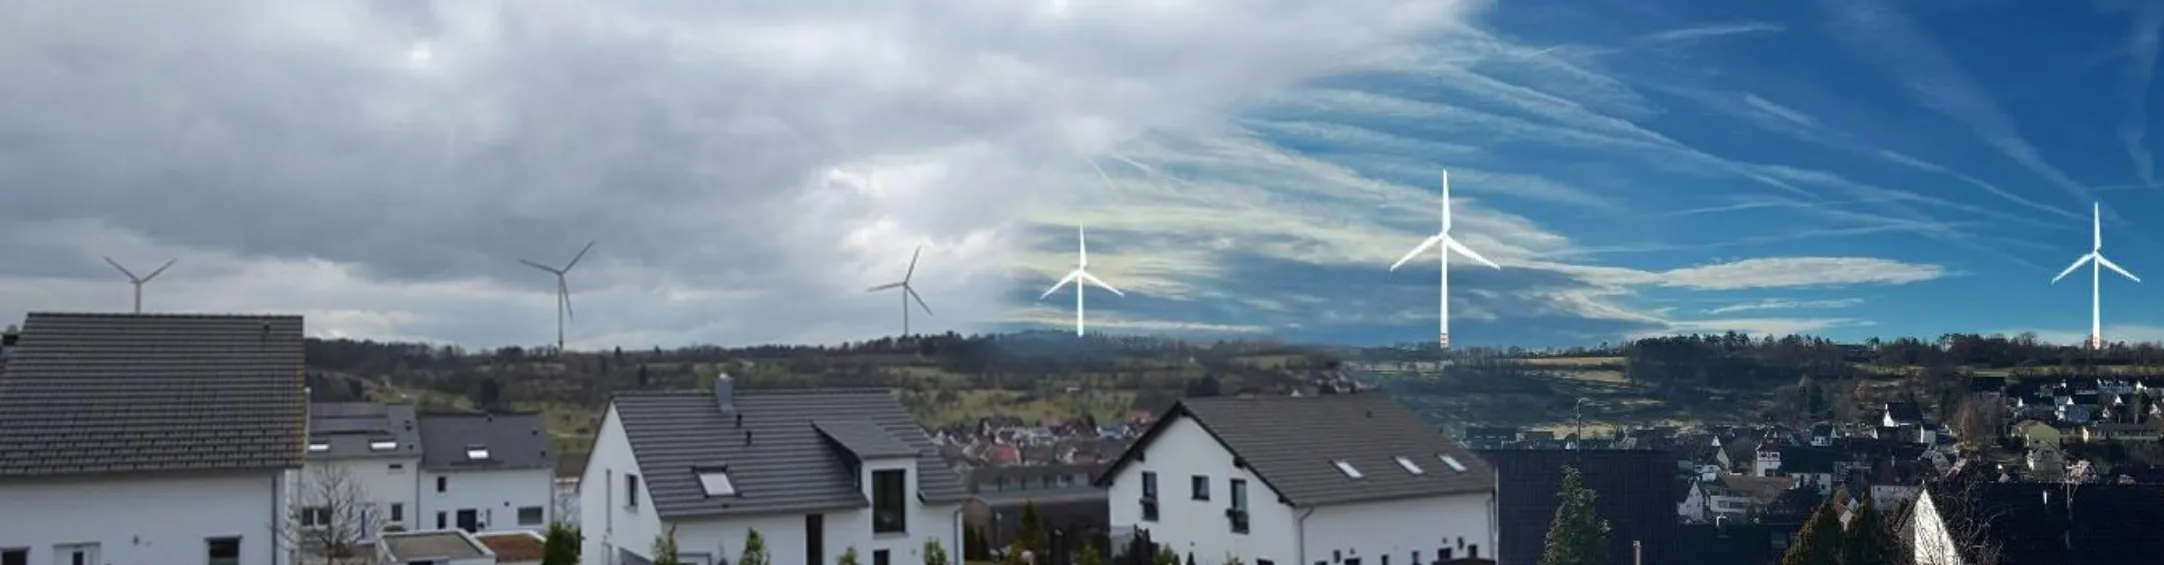
\includegraphics[
        width=\linewidth
    ]{figures/autokinetic-windmills.png}
    
    \caption{Fotomontage der Windparkprognosen. Diese Fotomontage zeigt die
    widersprüchlichen Prognosen zum Aussehen des geplanten Windparks. Links im
    wolkenverhangenen Bild die Darstellung der Stadtwerke Tübingen, rechts die
    dramatisierte Version des Vereins Freie Landschaft Ostelsheim e.V.}
    
    \label{fig:windpark}
\end{figure}

%%%%%%%%%%%%%%%%%%%%%%%%%%%%%%%%%%%%%%%%%%%%%%%%%%%%%%%%%%%%%%%%%%%%%%
\section{Diese Geschichte wiederholt sich?}

Um bis 2030 die Klimaschutzziele zu erreichen, sind zurzeit weitere 749
Windkraftanlagen in Baden-Württemberg im Verfahren, bereits genehmigt oder kurz
vor Inbetriebnahme \cite{umwelt2024}. Es ist zu erwarten, dass weitere
Konflikte auf Gemeindeebene folgen werden. Im Fall Ostelsheim reichten weder
offene Kommunikation noch der Kontakt zwischen den beteiligten Gruppen aus, um
Feindseligkeit zu verhindern, geschweige denn abzubauen. Die Nachwirkungen des
Konflikts sind bis heute spürbar, und gegenseitige Antipathien bestehen
weiterhin.

Die Theorie des realistischen Gruppenkonflikts legt nahe, dass sich Spannungen
durch das Verfolgen übergeordneter Ziele verringern lassen. Also an Zielen zu
arbeiten, die für beide Gruppen notwendig sind, nicht ignoriert werden können
und durch Anstrengungen beider Seiten erreicht werden können
\cite{jackson1993}. Ein Beispiel wären wirtschaftliche Anreize für die Nutzung
lokaler Energiequellen wie Wind- und Solarenergie zu verstärken, um die
Abhängigkeit von ausländischen Energieimporten, wie etwa aus Russland, zu
reduzieren und der Bevölkerung zu verdeutlichen. In Zukunft sollten Gemeinden,
die den Bau eines Windrades planen, diese Einsicht nutzen.

Dennoch bleibt die Frage, ob Konflikt und Streit nicht zum Wesen der Demokratie
gehören. Auch wenn die Entscheidung auf keiner wissenschaftlichen Grundlage
basierte: Vielleicht hat sie den Menschen, die sich von der Politik nicht ernst
genommen, bevormundet oder vergessen gefühlt haben, gezeigt, dass ihre Stimme
zählt.


%%%%%%%%%%%%%%%%%%%%%%%%%%%%%%%%%%%%%%%%%%%%%%%%%%%%%%%%%%%%%%%%%%%%%%
\clearpage
\bibliographystyle{apacite}
\bibliography{literatur}

\end{document}
